\documentclass{article}

\usepackage{fullpage}
\usepackage{amsmath}
\usepackage{amsfonts}
\usepackage{tikz}
\usepackage{cancel}
\usetikzlibrary{arrows}

\DeclareMathOperator{\atan2}{atan2}
\DeclareMathOperator{\tr}{Tr}

\begin{document}

\section{Homogenous Transformation}

Two frames $o_0 x_0 y_0 z_0$ and $o_1 x_1 y_1 z_1$ are related by
	the homogenous transformation, which sends frame 0 to frame 1:

\begin{align}
H & = \left[ \begin{matrix}
	0 & -1 & 0 & 1 \\
	1 & 0  & 0 & -1 \\
	0 & 0 & 1 & 0 \\
	0 & 0 & 0 & 1 
\end{matrix} \right] \label{eq:def-of-H}
\end{align}

A particle has velocity $v_1(t) = \left[ 3, 1, 0 \right]^T$ relative
	to the frame $o_1 x_1 y_1 z_1$.
Since the velocity and the frame are both constant, to find the velocity
	in frame zero, it suffices to express the vector $v_1$ in frame 0.
The inverse transformation is:

\begin{align*}
H^{-1} & = \left[ \begin{matrix}
	0 & 1 & 0 & -1 \\
	-1 & 0  & 0 & 1 \\
	0 & 0 & 1 & 0 \\
	0 & 0 & 0 & 1 
\end{matrix} \right]
\end{align*}

Since $v_1$ is a vector, the rotation is all that we need to consider.
Therefore, $v_0$ is:

\begin{align*}
\left[ \begin{matrix}
	0 & 1 & 0 \\
	-1 & 0 & 0 \\
	0 & 0 & 1 \end{matrix} \right]
\left[ \begin{matrix}
	3 \\
	1 \\
	0 \end{matrix} \right]
& =
\left[ \begin{matrix}
	1 \\
	-3 \\
	0 \end{matrix} \right]
\end{align*}

\section{Jacobian for 3-link Elbow Manipulator}

Compute the jacobian $J_{11}$ for the 3-link elbow manipulator of Example 4.9
	and show that it agrees with Equation (4.98).

From Eq. 4.58, if there are only revolute joints on a manipulator,
	
\begin{align}
J_{v_i} = z_{i-1} \times \left( o_n - o_{i-1} \right) \label{eq:def-of-Jvi}
\end{align}

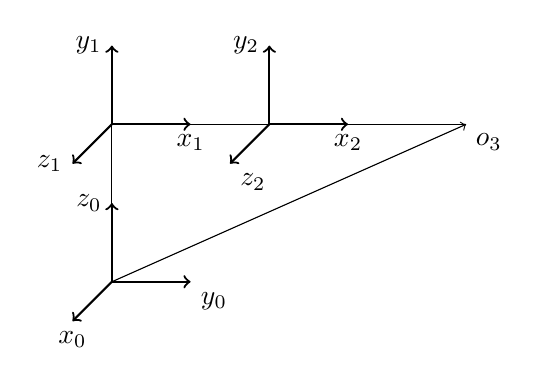
\begin{tikzpicture}
\coordinate (origin) at (0,0);
\draw[->, thick] (origin) to (-0.5,-0.5) node[below] (x0) {$x_0$};
\draw[->, thick] (origin) to (1,0) node[below right] (y0) {$y_0$};
\draw[->, thick] (origin) to (0,1) node[left] (z0) {$z_0$};

\coordinate (o1) at (0,2);
\draw[-] (origin) to (o1);
\draw[->, thick] (o1) to (1,2) node[below] (x1) {$x_1$};
\draw[->, thick] (o1) to (0,3) node[left] (y1) {$y_1$};
\draw[->, thick] (o1) to (-0.5, 1.5) node[left] (z1) {$z_1$};

\coordinate (o2) at (2,2);
\draw[-] (o1) to (o2);
\draw[->, thick] (o2) to (3,2) node[below] (x2) {$x_2$};
\draw[->, thick] (o2) to (2,3) node[left] (y2) {$y_2$};
\draw[->, thick] (o2) to (1.5, 1.5) node[below right] (z2) {$z_2$};

\coordinate (o3) at (4.5,2);
\node[below right] (end) at (o3) {$o_3$};
\draw[-] (o2) to (o3);

\draw[->] (origin) to (o3);

\end{tikzpicture}

Show that the determinant agrees with Equation (4.99).

\subsection{Computing the Forward Kinematics}

I will first compute the forward kinematics of the arm, with
	the geometric approach.

\paragraph{}
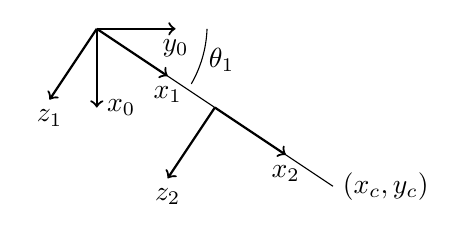
\begin{tikzpicture}

\coordinate(o0) at (0,0);
\draw[->, thick] (o0) to (1,0) node[below] (y0) {$y_0$};
\draw[->, thick] (o0) to (0,-1) node[right] (x0) {$x_0$};

\coordinate(o1) at (0,0);
\draw[->, thick] (o1) to (0.9,-0.6) node[below] (x1) {$x_1$};
\draw[->, thick] (o1) to (-0.6,-0.9) node[below] (z1) {$z_1$};

\coordinate(o2) at (1.5, -1);
\draw[-] (o0) to (o2);
\draw[->, thick] (o2) to (1.5+0.9,-0.6-1) node[below] (x2) {$x_2$};
\draw[->, thick] (o2) to (-0.6+1.5,-0.9-1) node[below] (z2) {$z_2$};

\coordinate(o3) at (3,-2);
\node[right] at (o3) (endeffector) {$(x_c, y_c)$};
\draw[-] (o2) to (o3);

\draw (1.2,-0.7) arc (-30:-2:1.5);
\node[right] at (1.3, -0.4) (theta1) {$\theta_1$};
\end{tikzpicture}


\subsection{Computing the Jacobian}

The first column of the jacobian is 

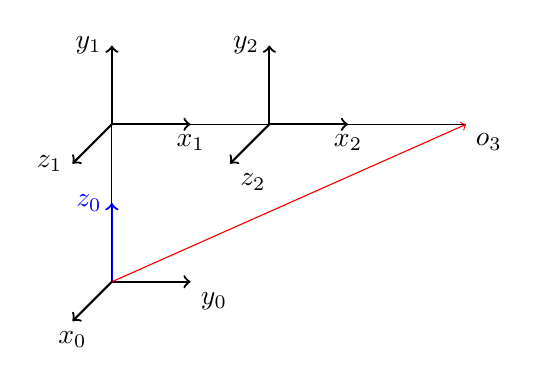
\begin{tikzpicture}
\coordinate (origin) at (0,0);
\draw[->, thick] (origin) to (-0.5,-0.5) node[below] (x0) {$x_0$};
\draw[->, thick] (origin) to (1,0) node[below right] (y0) {$y_0$};
\draw[->, thick, color=blue] (origin) to (0,1) node[left] (z0) {$z_0$};

\coordinate (o1) at (0,2);
\draw[-] (origin) to (o1);
\draw[->, thick] (o1) to (1,2) node[below] (x1) {$x_1$};
\draw[->, thick] (o1) to (0,3) node[left] (y1) {$y_1$};
\draw[->, thick] (o1) to (-0.5, 1.5) node[left] (z1) {$z_1$};

\coordinate (o2) at (2,2);
\draw[-] (o1) to (o2);
\draw[->, thick] (o2) to (3,2) node[below] (x2) {$x_2$};
\draw[->, thick] (o2) to (2,3) node[left] (y2) {$y_2$};
\draw[->, thick] (o2) to (1.5, 1.5) node[below right] (z2) {$z_2$};

\coordinate (o3) at (4.5,2);
\node[below right] (end) at (o3) {$o_3$};
\draw[-] (o2) to (o3);

\draw[->, color=red] (origin) to (o3);

\end{tikzpicture}

The cross product is:

\begin{align*}
z_0 \times (o_3 - o_0)
	& = \left[ \begin{matrix} 0 \\ 0 \\ 1 \end{matrix} \right]
	\times \left[ 
		\begin{matrix} 
			\cos \theta_1 (a_2 \cos \theta_2 + a_3 \cos ( \theta_2 + \theta_3))\\
			\sin \theta_1 (a_2 \cos \theta_2 + a_3 \cos ( \theta_2 + \theta_3))\\
			a_1 + (a_2 \sin \theta_2 + a_3 \sin (\theta_2 + \theta_3))
		\end{matrix} \right]\\
	& = 
	\left[ 
		\begin{matrix} 
			-\sin \theta_1 (a_2 \cos \theta_2 + a_3 \cos ( \theta_2 + \theta_3))\\
			\cos \theta_1 (a_2 \cos \theta_2 + a_3 \cos ( \theta_2 + \theta_3))\\
			0
		\end{matrix} \right]
\end{align*}

The second column of the jacobian is:

\begin{tikzpicture}
\coordinate (origin) at (0,0);
\draw[->, thick] (origin) to (-0.5,-0.5) node[below] (x0) {$x_0$};
\draw[->, thick] (origin) to (1,0) node[below right] (y0) {$y_0$};
\draw[->, thick] (origin) to (0,1) node[left] (z0) {$z_0$};

\coordinate (o1) at (0,2);
\draw[-] (origin) to (o1);
\draw[->, thick] (o1) to (1,2) node[below] (x1) {$x_1$};
\draw[->, thick] (o1) to (0,3) node[left] (y1) {$y_1$};
\draw[->, thick, color=blue] (o1) to (-0.5, 1.5) node[left] (z1) {$z_1$};

\coordinate (o2) at (2,2);
\draw[-] (o1) to (o2);
\draw[->, thick] (o2) to (3,2) node[below] (x2) {$x_2$};
\draw[->, thick] (o2) to (2,3) node[left] (y2) {$y_2$};
\draw[->, thick] (o2) to (1.5, 1.5) node[below right] (z2) {$z_2$};

\coordinate (o3) at (4.5,2);
\node[below right] (end) at (o3) {$o_3$};
\draw[-] (o2) to (o3);

\draw[->, color=red] (o1) to (o3);

\end{tikzpicture}

The cross product is:

\begin{align*}
z_1 \times (o_3 - o_1)
	& = \left[
		\begin{matrix} 
			\cos(\theta_1 - \pi/2) \\ \sin(\theta_1 - \pi/2) \\ 0 
		\end{matrix} \right]
	\times \left[ 
		\begin{matrix} 
			\cos \theta_1 (a_2 \cos \theta_2 + a_3 \cos ( \theta_2 + \theta_3))\\
			\sin \theta_1 (a_2 \cos \theta_2 + a_3 \cos ( \theta_2 + \theta_3))\\
			a_2 \sin \theta_2 + a_3 \sin (\theta_2 + \theta_3)
		\end{matrix} \right]\\
	& = \left[
		\begin{matrix} 
			\sin \theta_1 \\ - \cos \theta_1 \\ 0 
		\end{matrix} \right]
	\times \left[ 
		\begin{matrix} 
			\cos \theta_1 (a_2 \cos \theta_2 + a_3 \cos ( \theta_2 + \theta_3))\\
			\sin \theta_1 (a_2 \cos \theta_2 + a_3 \cos ( \theta_2 + \theta_3))\\
			a_2 \sin \theta_2 + a_3 \sin (\theta_2 + \theta_3)
		\end{matrix} \right]\\
	& = 
	\left[ 
		\begin{matrix} 
			- \cos \theta_1 
				\left(a_2 \sin \theta_2 + a_3 \sin (\theta_2 + \theta_3)\right)\\ 
			- \sin \theta_1 
				\left(a_2 \sin \theta_2 + a_3 \sin (\theta_2 + \theta_3)\right)\\ 
			\left(\cos^2 \theta_1 + \sin^2 \theta_1 \right)
				\left(a_2 \cos \theta_2 + a_3 \cos ( \theta_2 + \theta_3\right)
		\end{matrix} \right]\\
	& = 
	\left[ 
		\begin{matrix} 
			- \cos \theta_1 
				\left(a_2 \sin \theta_2 + a_3 \sin (\theta_2 + \theta_3)\right)\\ 
			- \sin \theta_1 
				\left(a_2 \sin \theta_2 + a_3 \sin (\theta_2 + \theta_3)\right)\\ 
			\left(a_2 \cos \theta_2 + a_3 \cos ( \theta_2 + \theta_3 \right)
		\end{matrix} \right]
\end{align*}

The third column of the jacobian is:

\begin{tikzpicture}
\coordinate (origin) at (0,0);
\draw[->, thick] (origin) to (-0.5,-0.5) node[below] (x0) {$x_0$};
\draw[->, thick] (origin) to (1,0) node[below right] (y0) {$y_0$};
\draw[->, thick] (origin) to (0,1) node[left] (z0) {$z_0$};

\coordinate (o1) at (0,2);
\draw[-] (origin) to (o1);
\draw[->, thick] (o1) to (1,2) node[below] (x1) {$x_1$};
\draw[->, thick] (o1) to (0,3) node[left] (y1) {$y_1$};
\draw[->, thick] (o1) to (-0.5, 1.5) node[left] (z1) {$z_1$};

\coordinate (o2) at (2,2);
\draw[-] (o1) to (o2);
\draw[->, thick] (o2) to (3,2) node[below] (x2) {$x_2$};
\draw[->, thick] (o2) to (2,3) node[left] (y2) {$y_2$};
\draw[->, thick, color=blue] (o2) to (1.5, 1.5) node[below right] (z2) {$z_2$};

\coordinate (o3) at (4.5,2);
\node[below right] (end) at (o3) {$o_3$};
\draw[-] (o2) to (o3);

\draw[->, color=red] (o2) to (o3);

\end{tikzpicture}

with the cross product:

\begin{align*}
z_2 \times (o_3 - o_2) 
	& = \left[ \begin{matrix}
		\sin \theta_1\\
		-\cos \theta_1\\
		0
	\end{matrix} \right]
	\times
	\left[ \begin{matrix}
		\cos \theta_1 a_3 \cos(\theta_2 + \theta_3) \\
		\sin \theta_1 a_3 \cos(\theta_2 + \theta_3) \\
		a_3 \sin(\theta_2 + \theta_3)
	\end{matrix} \right]\\
	& = \left[ \begin{matrix}
		- \cos \theta_1 a_3 \sin(\theta_2 + \theta_3)\\
		- \sin \theta_1 a_3 \sin(\theta_2 + \theta_3)\\
		\left( \sin^2 \theta_1 + \cos^2 \theta_1 \right)
			a_3 \cos (\theta_2 + \theta_3)
	\end{matrix} \right]
\end{align*}

The complete jacobian is therefore:

\begin{align}
J_{11} & = 
	\left[ \begin{matrix}
		-\sin \theta_1 (a_2 \cos \theta_2 + a_3 \cos ( \theta_2 + \theta_3))
			& 
			- \cos \theta_1 
				\left(a_2 \sin \theta_2 + a_3 \sin (\theta_2 + \theta_3)\right)
			&
		- \cos \theta_1 a_3 \sin(\theta_2 + \theta_3)\\
		\cos \theta_1 (a_2 \cos \theta_2 + a_3 \cos ( \theta_2 + \theta_3))
			& 
			- \sin \theta_1 
				\left(a_2 \sin \theta_2 + a_3 \sin (\theta_2 + \theta_3)\right) 
			&
			- \sin \theta_1 a_3 \sin(\theta_2 + \theta_3)\\
		0
			&		
			\left(a_2 \cos \theta_2 + a_3 \cos ( \theta_2 + \theta_3 \right)
			&
			a_3 \cos (\theta_2 + \theta_3)
	\end{matrix} \right]
\end{align}

\subsection{Determinant of the Jacobian}

$\det J_{11}$ is given by:

\begin{align*}
\det J_{11}
	& = 
	-\sin \theta_1 (a_2 \cos \theta_2 + a_3 \cos ( \theta_2 + \theta_3))
	\det \left[ \begin{matrix}
			- \sin \theta_1 
				\left(a_2 \sin \theta_2 + a_3 \sin (\theta_2 + \theta_3)\right) 
			&
			- \sin \theta_1 a_3 \sin(\theta_2 + \theta_3)\\
			\left(a_2 \cos \theta_2 + a_3 \cos ( \theta_2 + \theta_3 \right)
			&
			a_3 \cos (\theta_2 + \theta_3)
	\end{matrix} \right]\\
	& + \cos \theta_1 (a_2 \cos \theta_2 + a_3 \cos ( \theta_2 + \theta_3))
	\det \left[ \begin{matrix}
		(a_2 \cos \theta_2 + a_3 \cos ( \theta_2 + \theta_3 ))
		&
		a_3 \cos (\theta_2 + \theta_3)\\
		- \cos \theta_1 
			\left(a_2 \sin \theta_2 + a_3 \sin (\theta_2 + \theta_3)\right)
			&
		- \cos \theta_1 a_3 \sin(\theta_2 + \theta_3)
	\end{matrix} \right]\\
	& = \left( a_2 \cos \theta_2 + a_3 \cos (\theta_2 + \theta_3) \right)\\
	&
		- \sin \theta_1
			\left( - a_3 \cos(\theta_2 + \theta_3)
					\sin \theta_1 (a_2 \sin \theta_2 + a_3 \sin (\theta_2 + \theta_3))
					+ a_3 \sin \theta_1 \sin(\theta_2 + \theta_3)
					(a_2 \cos \theta_2 + a_3 \cos (\theta_2 + \theta_3)) \right)\\
	&	\cos \theta_1
			\left( - \cos \theta_1 a_3 \sin(\theta_2 + \theta_3)
				(a_2 \cos \theta_2 + a_3 \cos(\theta_2 + \theta_3))
				+ a_3 \cos(\theta_2 + \theta_3)
				\cos \theta_1 (a_2 \sin \theta_2 + a_3 \sin(\theta_2 + \theta_3))
			\right)\\
	& = a_3 \left( a_2 \cos \theta_2 + a_3 \cos (\theta_2  +\theta_3) \right)\\
	& (\sin^2 \theta_1 
		\left(
			\cos(\theta_2 + \theta_3)(a_2 \sin \theta_2 + a_3 \sin (\theta_2 + \theta_3)
			- \sin(\theta_2 + \theta_3)(a_2 \cos \theta_2 + a_3 \cos (\theta_2 + \theta_3)
		\right)\\
	& + \cos^2 \theta_1 
		\left(
			\cos(\theta_2 + \theta_3)(a_2 \sin \theta_2 + a_3 \sin (\theta_2 + \theta_3)
			- \sin(\theta_2 + \theta_3)(a_2 \cos \theta_2 + a_3 \cos (\theta_2 + \theta_3)
		\right) )\\
	& = a_3 \left( a_2 \cos \theta_2 + a_3 \cos (\theta_2  +\theta_3) \right)
		\left(
			\cos(\theta_2 + \theta_3)(a_2 \sin \theta_2 + \cancelto1{a_3 \sin (\theta_2 + \theta_3)})
			- \sin(\theta_2 + \theta_3)(a_2 \cos \theta_2 + \cancelto1{a_3 \cos (\theta_2 + \theta_3)})
		\right)\\
	& = a_2 a_3 \left( a_2 \cos \theta_2 + a_3 \cos (\theta_2  +\theta_3) \right)
		\left(
			\cos(\theta_2 + \theta_3) \sin \theta_2
			- \sin(\theta_2 + \theta_3) \cos \theta_2
		\right)\\
	& = a_2 a_3 \left( a_2 \cos \theta_2 + a_3 \cos (\theta_2  +\theta_3) \right)
		\sin ( \theta_2 + \theta_3 - \theta_2 )\\
	& = a_2 a_3 \sin \theta_3 \left( a_2 \cos \theta_2 + a_3 \cos (\theta_2  +\theta_3) \right)
\end{align*}
		


\section{The Pseudoinverse and the Solution Space}
Suppose that $\dot{q}$ is a solution the the equation (\ref{eq:inverse-kinematics}) below:

\begin{align}
	\xi & = J \dot{q} \label{eq:inverse-kinematics}
\end{align}

\subsection{Finding Other Solutions}

I will show that $\dot{q} + \left( 1 - J^+J \right) b$ is also a solution to
	equation \ref{eq:inverse-kinematics} for any $b \in \mathbb{R}^n$.

Recall the definition of $J^+$:

\begin{align}
	J^+ & \equiv J^T (J J^T)^{-1}
\end{align}

Note that $J J^+ = 1$.
Therefore, if $\dot{q}$ is such that $\xi = J \dot{q}$, then:

\begin{align}
	J \left( \dot{q} + \left( 1 - J^+J \right) b \right) & = \nonumber \\
	J \dot{q} + J b - J J^+ (J b) & = \nonumber \\
	J \dot{q} + J b - J b & = \nonumber \\
	J \dot{q} & = \xi \nonumber
\end{align}

Therefore, for all $b \in \mathbb{R}^n$, if (\ref{eq:inverse-kinematics}) holds,
	then (\ref{eq:inverse-kinematics-with-b}) holds, as shown below:

\begin{align}
	J \left( \dot{q} + (1 - J^+ J ) b \right) & = \xi 
		\label{eq:inverse-kinematics-with-b}
\end{align}

\subsection{Showing that $b = 0$ minimizes the resulting joint velocities}

\begin{align}
J^+ & = J^T (J J^T)^{-1} \\
{J^+}^T & = (J J^T)^{-1} J \\
{J^+ }^T J^+ & = (J J^T)^{-1} 
\end{align}

The resuliting joint velocities are $J^+ \xi + (1 - J^+ J)b$.
	for some $b \in \mathbb{R}^n$.
This is $J^+ (\xi - J b) + b$.

\begin{align*}
\left\lVert \dot{q} \right\rVert^2
	& = (J^+ \xi + (1 - J^+ J) b)^T (J^+ \xi + (1 - J^+ J) b) \\
	& = (\xi^T {J^+}^T
		+ b^T (1 - J^T {J^+}^T))(J^+ \xi + (1 - J^+ J) b) \\
	& = \xi^T (J J^T)^{-1} \xi + \cancelto1{\xi^T (J J^T)^{-1} (J b)}
		- \cancelto1{\xi^T (J J^T)^{-1} (J b)}\\
	& + \cancelto2{(J b)^T (J J^T)^{-1} \xi} + b^T b 
		- (J b)^T (J J^T)^{-1} (J b)\\
	& - \cancelto2{(J b)^T (J J^T)^{-1} \xi} 
		- \cancelto3{(J b)^T (J J^T)^{-1} (J b)}
		+ \cancelto3{(J b)^T (J J^T)^{-1} (J b)}\\ 
	& = \xi^T (J J^T)^{-1} \xi + b^T b - (J b)^T (J J^T)^{-1} (J b)\\
	& = \xi^T (J J^T)^{-1} J J^T (J J^T)^{-1} \xi
	+ b^T b - b^T J^T (J J^T)^{-1}  J J^T (J J^T)^{-1} J b\\
\left\lVert \dot{q} \right\rVert^2
	& = \left\lVert J^+ \xi \right\rVert^2
		+ \left\lVert b \right\rVert^2
		- \left\lVert J^+ J b \right\rVert^2
\end{align*}

Since the operator $J^+ J$ projects $b$ onto the nullspace of $J$,
	the norm of $J^+ J b$ will always be less than the norm of $b$.
Therefore, the quantity $\left\lVert b \right\rVert^2 
	- \left\lVert J^+ J b \right\rVert^2$
	is nonnegative, and thus is minimized by setting $b = 0$.

%	It is a property of norms that:
%	
%	\begin{align}
%	\left\lVert J^+ J b \right\rVert^2
%		& \leq \left\lVert J^+ J \right\rVert^2 \left\lVert b \right\rVert^2
%	\end{align}
%	
%	Therefore, 
%	
%	\begin{align}
%	\left\lVert b \right\rVert^2
%		- \left\lVert J^+ J b \right\rVert^2
%		& \leq \left\lVert b \right\rVert^2 
%			\left( 1 - \left\lVert J^+ J \right\rVert^2 \right)
%	\end{align}

\section{Exploiting the null-space}

In the previous section, the expression $(1 - J^+ J) b$ projects the vector $b$ 
	onto the null space of the jacobian.
While choices of $b$ do not alter the end-effector velocity, they do alter the joint
	velocities.
The choice of $b$ lets me chose among different joint velocities which satisfy
	the end-effector velocity constraint.

Since I can use $b$ to chose among many different joint velocity configurations,
	I can chose $b$ to satsify several objectives.

\begin{enumerate}
\item
I showed in the previous section that a choice of $b = 0$ will minimize the total magnitude
	of the joint velocity vector.
\item
I may be interested in minimizing something else, for example, the joint velocity
	of a slow joint.
A different choice of $b$ may minimize that velocity.
\item
I may also want to keep my joint velocity values within a certain range.
This will be a linear programming problem, which can potentially be computationally
	difficult.
\end{enumerate}

\section{Path Planning with Artificial Potential Fields}

A motion planner that uses artificial potential fields is guarenteed to reach its
	goal if there are no local minima.
If there is a unique local minimum, then the gradient descent algorithm is guarenteed
	to reach it.
However, if there are local minima, then the gradient descent algorithm can get stuck there,
	and probabilistic methods need to be used to extract it from the local minimum.

\section{Probabilitic Path Planners vs. Deterministic Path Planners}

\subsection{Simple Workspaces}

In a workspace with few obstacles, probabilistic planners will not be able to take
	advantage of this fact, and will explore the space as usual, recieving fewer
	rejected samples and eventually producing a path to the goal.

However, artificial potential fields will quickly produce a path which goes directly
	to the goal.

\subsection{Irregular Workspaces}

Probabilistic Path Planners are well-equipped to deal with irregular workspaces.
If there are many different intermediate configurations, the path planner
	may sample them.

However, Artificial Potential Fields may yield local minima along the path to the
	goal in an irregular workspace.
These local minima may be escaped with probabilistic processes, or other processes.

\subsection{High-Dimensional Workspaces}

High-Dimensional Workspaces are difficult to sample with a probabilitics
	path planner.
As the number of dimensions increases, exponentially more samples are required to have
	a reasonable map of the space.
The narrow passage problem becomes more acute in higher dimensions as well, because
	large regions have far more volume.

Artificial Potential Fields will not be significantly affected by the increase
	in dimensionality.
The distance to the nearest obstacle, which could be approximated as the distance to the
	nearest vertex, will not become significiantly more difficult to compute.
The increase in dimensionality can slow it down only polynomially.
Therefore constructing the artificial potential field will not be significantly more
	difficult in higher dimensions.

\section{Narrow Passage Problem}

The Narrow Passage problem is a drawback of probabilitic planners.
If there are two regions of large volume connected by a region of small volume,
	uniform random sampling is unlikely to sample within the region of small volume.
This problem is especially acute at high configuration space dimensions.
The probabilitic motion planner will treat the two regions as discontinuous, and finding
	the path will be very difficult unless sampling is done more intelligently.

The game \emph{Operation} will cause a narrow passage problem in a manipulator.
The goal is to pick up a small plastic game piece embedded in a hole with metal tweezers, 
	without touching the tweezers to the side of the hole.
Very few configurations get the tweezers right through to the game piece.
If one is uniformly sampling, then these may be very difficult to find.
However, if one decides to sample more around the goal, then the configurations may be
	found.

\section{Using Motion Planners to solve Manipulation Problems}

The goal of motion planning is to find a good path through the configuration space which
	does not intersect any obstacles.
However, when one wants to manipulate objects, one needs to intersect the object which
	one is manipulating, and exert forces on it.
Motion Planning does not account for this.

A motion planner trying to pick up an object will try to place the manipulator exactly around
	the object.
This configuration has very little tolerance for error, and constitutes a narrow passage.
The motion planner does not encode the fact that the object will tolerate some squeezing 
	forces applied to it, and cannot take advantage of this to make its planning easier.
Therefore motion planners are not good for direct manipulation.

\section{Which robots use motion planners?}

Home robots are more likely to use motion planners than industrial robots, because an industrial
	robot operates within a highly structured and predicatable environment while a home
	robot must adjust to a constantly changing environment.

Since industrial robots typically will only perform a single action within their lifecycle,
	their action can be efficiently hand-engineered.
Technicians can manually make an efficient trajectory one time, and then direct the industrial
	robot to repeat that trajectory.

Home robots, however, are deposited in an unfamiliar environment that they need to explore.
Even when they do explore, it is constantly changing, as new obstacles are added.
Therefore, the robot needs to do its own path planning, and needs to come up with
	new paths to adjust to new situations.


%	\section{Exponentials}
%	
%	Given a square matrix $A$, $e^A$ is defined as the power series
%		$1 + A + \frac{A^2}2 + \dots + \frac{A^n}{n!} + \dots$
%	Suppose $S \in so(3)$.
%	Show that $e^S \in SO(3)$
%	
%	\begin{align}
%		{e^A}^T & = e^{A^T}\\
%		e^A e^B & = e^{A + b} \text{ provided $[A,B] = 0$}\\
%		\det(e^A) &  = e^{\tr A}
%	\end{align}
%	
%	Since $A \in so(3)$, $A^T A = A A^T = I$, and therefore $A$ and $A^T$ commute.
%	Therefore,
%	
%	\begin{align}
%		{e^A}^T e^A & = e^{A + A^T}
%	\end{align}

\end{document}
